% begin module limits-one-sided-def
\begin{frame}
\begin{definition}[\only<handout:1| -2>{\vphantom{Right}Left}\only<handout:2| 3->{\vphantom{Left} \alert<3>{Right}}-hand Limit ]
We write
\[
\lim_{x\rightarrow a^{\only<handout:1| -2>{-}\only<handout:2| 3->{\alert<3>{+}}}\phantom{+} }f(x) = L \quad \quad \quad \text{or} \quad \quad \quad  \lim\limits_{\substack{x\rightarrow a \\ x\only<handout:1| -2>{<}\only<handout:2| 3->{\alert<3>{>}}a
}}f(x)=L
\]
and say the \alt<handout:1| -2>{\vphantom{right}left}{\alert<3>{\vphantom{left}right}}-hand limit of $f(x)$ as $x$ approaches $a$ is equal to $L$ \\  if we can make the values of $f(x)$ arbitrarily close to $L$ by taking $x$ to be sufficiently close to and \only<handout:1| -2>{\vphantom{greater}less}\only<handout:2| 3->{\alert<3>{\vphantom{less}greater}} than $a$. 
\end{definition}
\begin{columns}[c]
\column{.5\textwidth}
\psset{xunit=0.8cm, yunit=0.8cm}
\begin{pspicture}(-0.6, -0.6)(4.6,4.8) 
\psaxes[ticks=none, labels=none]{<->}(0,0)(-0.5,-0.55)(4.5,4.5)
\tiny
%\psLabels{4.5}{4.5}
%Function formula: 4+1/6 ((x)^{3})-5/8 ((x)^{2})-3/4 (x) 
\psplot[linecolor=red, plotpoints=1000]{-0.49}{4}{x -0.75 mul x 2 exp -0.625 mul x 3 exp 0.166667 mul 4 add add add }
\rput[l] (1,3){$y=f(x)$}
\psline[linecolor=black](2.4,0)(2.4,0.904)
\rput[r](2.35, 0.45){$f(x)$}
\rput[t](2.4, -0.1){$x$}
\psline[linewidth=1pt]{->}(2.5, -0.15)(3.1,-0.15)
\psline[linecolor=black](3.2,0)(3.2,0.661333333)
\rput[l](3.25, 0.3){$L$}
\rput[t](3.2, -0.1){$a$}
\end{pspicture} 
%\ 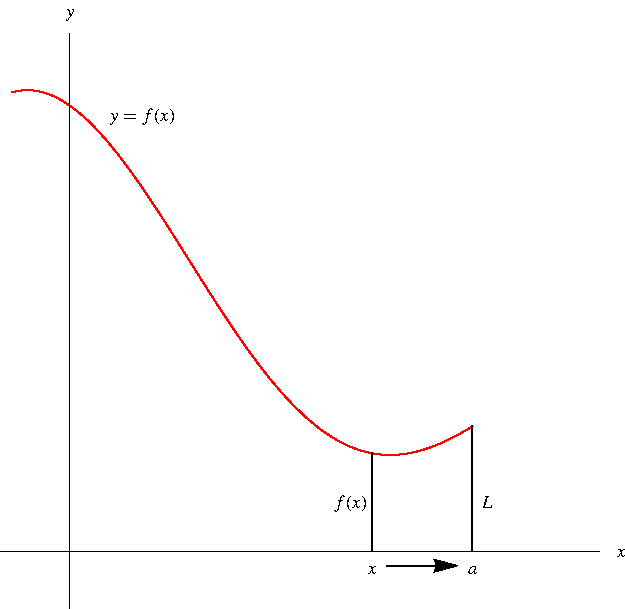
\includegraphics[height=4cm]{limits/pictures/02-02-leftlim.pdf}%
\column{.5\textwidth}
\uncover<handout:2| 3->{%
\psset{xunit=0.8cm, yunit=0.8cm}
\begin{pspicture}(-0.6, -0.6)(4.6,4.8)  
\psaxes[ticks=none, labels=none]{<->}(0,0)(-0.5,-0.5)(4.5,4.5)\tiny
%\psLabels{4.5}{4.5}
%Function formula: 3+1/9 ((x)^{3})-1/3 ((x)^{2})-1/2 (x) 
\psplot[linecolor=red, plotpoints=1000]{-0.49}{4}{x -0.5 mul x 2 exp -0.333333 mul x 3 exp 0.111111 mul 3 add add add }
\rput[l] (0.5,3){$y=f(x)$}
\psline[linecolor=black](2.2,0)(2.2,1.469777778)
\rput[l](2.25, 0.7){$f(x)$}
\rput[t](2.2, -0.1){$x$}
\psline[linewidth=1pt]{->}(2.1, -0.15)(1.5,-0.15)
\psline[linecolor=black](1.4,0)(1.4,1.951555556)
\rput[r](1.35, 0.9){$L$}
\rput[t](1.4, -0.1){$a$}
\end{pspicture}
%\ 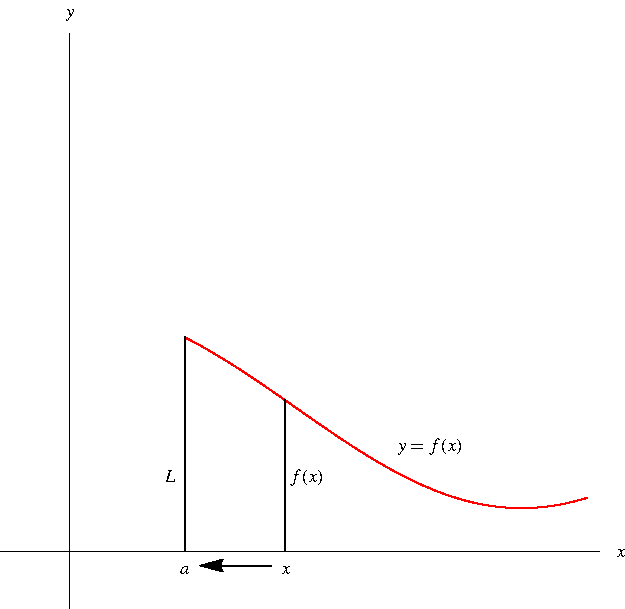
\includegraphics[height=4cm]{limits/pictures/02-02-rightlim.pdf}%
}%
\end{columns}
\uncover<handout:2| 2->{%
We can define a \alert<3>{right}-hand limit similarly.
}%
\end{frame}
% end module limits-one-sided-def